\chapter{Marco teórico}

\section{Antecedentes bibliográficos}

Partimos el corpus en seis ejes. No todos pesan lo mismo para el score. La tabla junta el hallazgo, qué pieza del score toca, y el hueco que nos queda.

\begin{table}[H]
  \centering
  \caption{Síntesis de los seis ejes}
  \label{tab:ejes}
  \footnotesize
  \begin{tabular}{@{}p{0.08\textwidth}p{0.28\textwidth}p{0.22\textwidth}p{0.28\textwidth}@{}}
    \toprule
    Eje & Papers & Aporte & Hueco \\
    \midrule
    E1 & Casas; Mainas; Santos y Casas & El contrato como artefacto. Mainas alimenta S & Sin Service Domain \\
    E2 & Shvaiko y Euzenat & La taxonomía de E & Sin REST ni banca \\
    E3 & El Bayadh; Chandrasekaran; Santos Sousa; He; Schneider; Hertling & S por similitud. C solo de paso & Sin OpenAPI bancario \\
    E4 & Schmidt; Lu; Kotstein; Oberle & Dominio hacia interfaz & El segundo archivo sigue siendo una API \\
    E5 & Ehsan; Golmohammadi; Otieno; Tanveer; Vitorino & Queda fuera. Es testing & No es el AlignmentScore \\
    E6 & Mahanra Rao & S parcial, por ranking & Elegir un servicio no es alinearlo con BIAN \\
    \bottomrule
  \end{tabular}
\end{table}

\subsection{OpenAPI como contrato}

Casas et al.\ \cite{Casas2021} revisan 47 artículos de 2011 a 2020. OpenAPI queda como la descripción REST que una máquina puede leer. El uso que encuentran es generar código, probar y gobernar. El 68\,\% propone herramientas y el 43\,\% mejora la documentación. En esos 47 el contrato no queda al lado de un Service Domain. Mainas et al.\ \cite{Mainas2023} anotan el contrato (\texttt{x-refersTo}, \texttt{x-kindOf}, \texttt{x-mapsTo}), lo pasan a RDF y consultan con SPARQL más de 300 especificaciones de SwaggerHub. Un YAML de más de 200 líneas les llevó más de un segundo. No definen un SemanticScore, y el corpus es SwaggerHub, no banca. Santos y Casas \cite{SantosCasas2025}, con \textit{design science}, catalogan 59 métricas de API Gateway (latencia, tráfico, errores) en 68 productos. Eso es calidad en producción. No es el cruce del YAML con un Service Domain.

\subsection{Emparejamiento de esquemas}

Shvaiko y Euzenat \cite{Shvaiko2005} ordenan el \textit{schema matching} en tres cortes: exacto o aproximado; evidencia sintáctica, semántica o externa; elemento o estructura. El trabajo es anterior a OpenAPI y a JSON Schema. El StructuralScore usa el corte aproximado. La evidencia es el nombre, la ruta y el verbo. El grano es la operación, no el archivo entero. \textit{Paths}, operaciones y \textit{schemas} se leen contra behaviors y business objects. No traen un corpus bancario. La métrica que se puede repetir sobre ese par la fijamos nosotros, en el capítulo III.

\subsection{Similitud y ontologías}

El Bayadh et al.\ \cite{ElBayadh2015} separan la alineación ontológica en terminológica, estructural, extensional y semántica. Avistan que una sola medida no basta y que una combinación fija puede quedar corta. Por eso S, E y C no se sustituyen entre sí, y los pesos iguales del AlignmentScore se acompañan de dos juegos de sensibilidad. Chandrasekaran y Mago \cite{Chandrasekaran2022} recorren la similitud desde WordNet hasta los \textit{transformers}. Santos Sousa et al.\ \cite{SantosSousa2026} listan tres límites de los \textit{embeddings} en ontology matching: hace falta supervisión, la escala pesa, y hay correspondencias que no son uno a uno.

Tres trabajos recientes dicen qué encoder usar y qué no ajustar. He et al.\ \cite{He2022} fine-tunean BERT (BERTMap) sobre el texto de la ontología y reparan el alineamiento con la estructura. Schneider et al.\ \cite{Schneider2023} codifican la etiqueta con un \textit{sentence transformer} ya entrenado y comparan por coseno, sin ajuste. Hertling y Paulheim \cite{Hertling2023} le preguntan a un modelo grande, con pocos ejemplos, si dos entidades coinciden. Nos quedamos con el coseno de Schneider et al. No copiamos el ajuste de He et al.: no hay una ontología BIAN etiquetada. El par no lo arma un chat.

\subsection{Dominio e interfaz}

Schmidt y Thiry \cite{Schmidt2020} revisan 27 estudios primarios, de 715 registros entre 2013 y 2019, sobre cómo identificar microservicios con MDE y DDD. Un Service Domain puede ser la referencia de negocio y la API la capa que lo expone. Esa revisión no calcula un desfase. Lu et al.\ \cite{Lu2024} agrupan microservicios parecidos con GloVe sobre el OpenAPI entero. Kotstein y Decker \cite{Kotstein2024} ajustan BERT con 2\,321 especificaciones para señalar un endpoint a partir de una pregunta. Oberle y Bauernhansl \cite{Oberle2024} comparan TF-IDF, word2vec, fastText y embeddings sobre 326 endpoints de un MES, con corte de expertos. En los tres el segundo archivo también es una API. Nosotros ponemos al lado un Service Domain.

\subsection{Lo que no entra}

Ehsan et al.\ \cite{Ehsan2022} cubren 16 artículos de testing RESTful. La métrica que domina es el \textit{code coverage}. Golmohammadi et al.\ \cite{Golmohammadi2024} leen 92 papers que generan casos sobre endpoints ya vivos. Otieno y Araka \cite{Otieno2026} ponen aprendizaje automático en las pruebas y se quejan de datasets chicos. Tanveer et al.\ \cite{Tanveer2025} van a vulnerabilidades. Vitorino et al.\ \cite{Vitorino2025}, a datos adversariales. Aquí OpenAPI es la entrada de una prueba. En esta tesis es el artefacto que se contrasta con el dominio. Mahanra Rao et al.\ \cite{MahanraRao2025} revisan 25 estudios (2020--2024) que usan BERT para elegir un servicio según su QoS. El ranking no es el AlignmentScore.

\section{Bases teóricas}

El StructuralScore se apoya en Shvaiko y Euzenat \cite{Shvaiko2005}: correspondencia entre esquemas, no un clasificador. El aviso de El Bayadh et al.\ \cite{ElBayadh2015} justifica no fiar el expediente a una sola medida. El SemanticScore de esta corrida es el coseno de un encoder de frases ya entrenado \cite{Schneider2023,Reimers2019}, no un BERT ajustado a BIAN \cite{He2022} ni una pregunta a un modelo generativo \cite{Hertling2023}.

El Bayadh separa cuatro familias. La terminológica es el S léxico, y en el piloto se queda entre 0,00 y 0,03: el YAML está en portugués y el dominio en inglés. La estructural es E. La semántica es el coseno de MiniLM. La extensional pediría filas de datos, movimientos, saldos reales. El archivo no las trae. Trae el contrato.

Mainas et al.\ \cite{Mainas2023} pasan el YAML a RDF, con una ontología REST. OE1 no hace eso. Deja una fila por operación. El vocabulario del score sale de esa tabla y del dominio ya normalizado. No sale de un texto suelto.

Dado un contrato y un Service Domain emparejado, el procedimiento normaliza, calcula S, E y C, y junta

\[
\mathrm{AlignmentScore} = \alpha S + \beta E + \gamma C, \qquad \alpha+\beta+\gamma = 1.
\]

En la corrida oficial $\alpha = \beta = \gamma = 1/3$. La sensibilidad usa $(0{,}50,\ 0{,}30,\ 0{,}20)$ y $(0{,}20,\ 0{,}50,\ 0{,}30)$ sin cambiar el número oficial. El nivel es Alta si el score llega a 0,80, Media entre 0,60 y 0,79, Baja entre 0,40 y 0,59, y Nula por debajo de 0,40. Esos cortes no se aprenden.

CoverageScore no es el \textit{code coverage} de las pruebas \cite{Ehsan2022}. Es la fracción de tags \texttt{CR} y \texttt{BQ} del Service Domain que recibieron al menos un par. S se promedia solo sobre los pares que el greedy dejó. Las operaciones del contrato que se quedaron solas entran en E como cero, y no entran en S.

\section{Definición de términos}

Abajo, el vocabulario del score. Alineación es el cruce entre el archivo y el dominio. No nombra al banco.

\begin{table}[H]
  \centering
  \caption{Términos que usa el modelo}
  \label{tab:terminos}
  \small
  \begin{tabular}{@{}p{0.28\textwidth}p{0.64\textwidth}@{}}
    \toprule
    Término & Qué significa aquí \\
    \midrule
    Contrato OpenAPI & YAML o JSON (OpenAPI 3.x, o Swagger 2 cuando el estándar no migró) con \textit{paths}, operaciones y \textit{schemas}. \\
    Service Domain & Unidad de negocio BIAN: behaviors, business objects y relaciones de control. \\
    Behavior & Acción de negocio definida en el Service Domain. \\
    Business object & Entidad del dominio (una orden de pago, una cuenta) referida en el modelo. \\
    SemanticScore (S) & Parecido de significado entre los textos emparejados, en $[0,1]$. \\
    StructuralScore (E) & Correspondencia de nombre, ruta, verbo y profundidad, en $[0,1]$. No es una métrica de \textit{runtime}. \\
    CoverageScore (C) & Fracción de tags \texttt{CR}/\texttt{BQ} del dominio que recibieron par, en $[0,1]$. \\
    AlignmentScore & $(S+E+C)/3$ en la corrida oficial, con nivel Alta, Media, Baja o Nula. \\
    Schema matching & Correspondencia entre esquemas. Base de E \cite{Shvaiko2005}. \\
    Alineación & Correspondencia estructural y semántica entre el contrato y un Service Domain. \\
    Desalineación & Una de las cuatro de la tipología del capítulo I: estructural, semántica, de modelado, o de verbo y ruta. \\
    Instancia & Un contrato ya elegido contra un Service Domain ya elegido. I1 es \texttt{accounts} 2.4.2 contra Savings Account. No es el producto de los 38 YAML por los 258 dominios. \\
    Tag CR / BQ & Etiqueta del YAML de BIAN. CR es el registro de control del dominio. BQ califica un behavior, como Charge o Deposit. C es la fracción de esos tags que recibió al menos un par. \\
    Nivel & Alta, Media, Baja o Nula, con cortes fijos. No es una clase aprendida. \\
    \bottomrule
  \end{tabular}
\end{table}

\section{Brecha}

Los veinte papers del Anexo~\ref{anexo:papers}, leídos en cruz, dejan cinco cosas distintas. Casas et al.\ \cite{Casas2021} muestran el formato en 47 artículos, y Mainas et al.\ \cite{Mainas2023} prueban que el YAML se puede anotar. Shvaiko y Euzenat \cite{Shvaiko2005} dejan la taxonomía para cruzar esquemas. El Bayadh et al.\ \cite{ElBayadh2015} avisan que una medida no basta, y Santos Sousa et al.\ \cite{SantosSousa2026} dicen dónde fallan los embeddings: supervisión, escala, y pares que no son uno a uno. Schmidt y Thiry \cite{Schmidt2020} separan el dominio de la interfaz. BIAN puede ocupar ese lugar de referencia. Ehsan et al.\ \cite{Ehsan2022} y Golmohammadi et al.\ \cite{Golmohammadi2024} usan el contrato para probar APIs vivas. Mahanra Rao et al.\ \cite{MahanraRao2025} rankean servicios por calidad de servicio.

Casas y Mainas se quedan en el contrato. Shvaiko y El Bayadh no traen un YAML de banco. Schmidt separa el dominio de la interfaz y no calcula el desfase. Nosotros ponemos el Service Domain al lado del archivo y guardamos el AlignmentScore, para que otro pueda repetir el número.

\begin{table}[ht]
  \centering
  \caption{Vacíos V1 a V5}
  \label{tab:vacios}
  \footnotesize
  \begin{tabular}{@{}p{0.22\textwidth}p{0.34\textwidth}p{0.34\textwidth}@{}}
    \toprule
    Vacío & De dónde sale & Qué hacemos con eso \\
    \midrule
    V1. OpenAPI y BIAN juntos & El review no estudia los dos artefactos en banca & El objeto sigue siendo el contrato. BIAN es la referencia, y ese cruce no está en el review \\
    V2. Una métrica sola no alcanza & E2 y E3 aportan técnicas sueltas & S, E, C y el AlignmentScore \\
    V3. Cobertura & El matching ontológico habla de cobertura, no de business objects BIAN dentro del YAML & CoverageScore \\
    V4. Un procedimiento que se repita & Mainas et al.\ arman RDF. No dejan un score ni un nivel & El prototipo del capítulo III \\
    V5. Antes del despliegue & E5 y E6 miran runtime o ranking & El score es documental \\
    \bottomrule
  \end{tabular}
\end{table}

\begin{figure}[ht]
  \centering
  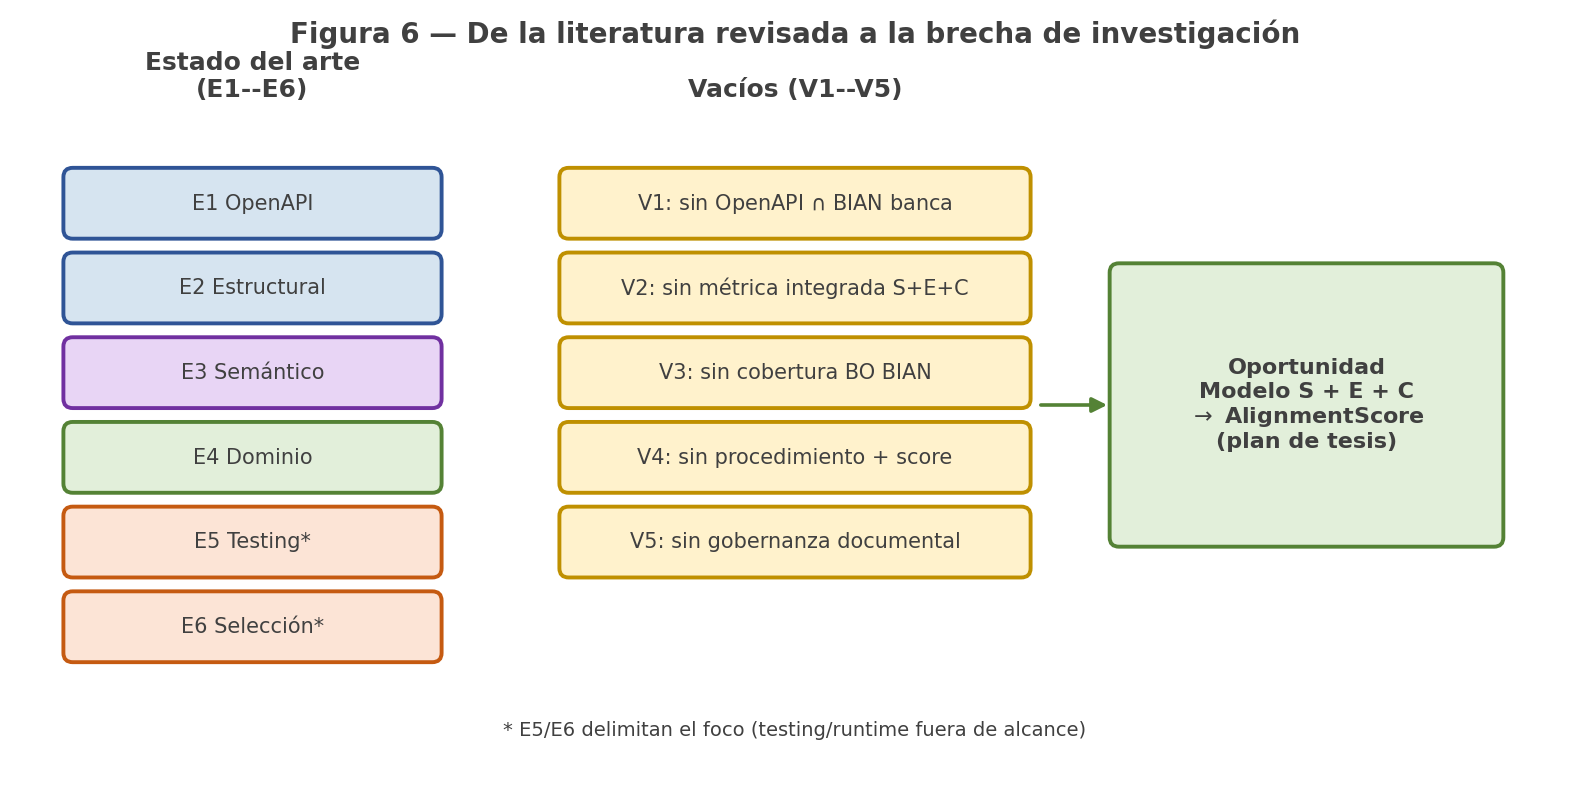
\includegraphics[width=0.92\textwidth]{Figura_06_Brecha}
  \caption{De los ejes E1--E6 a los vacíos V1--V5}
  \label{fig:brecha}
\end{figure}

\begin{figure}[ht]
  \centering
  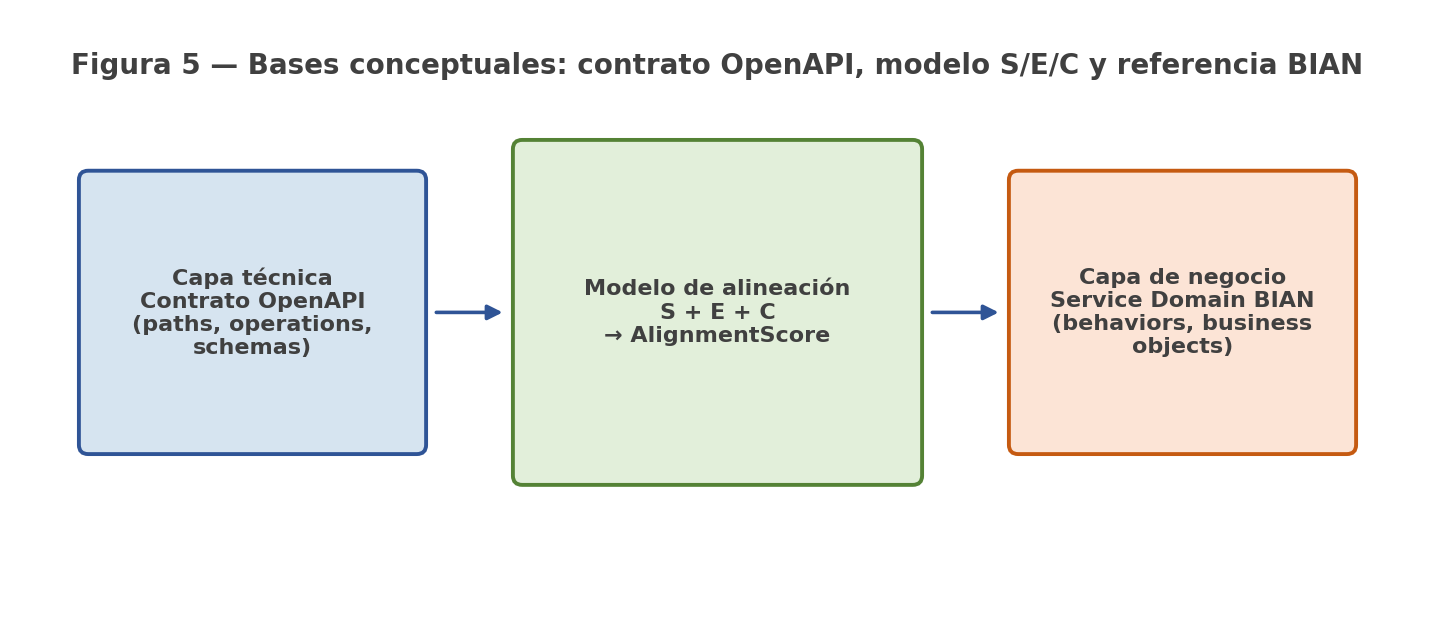
\includegraphics[width=0.88\textwidth]{Figura_05_Bases_Conceptuales}
  \caption{Contrato OpenAPI, Service Domain y modelo S/E/C}
  \label{fig:bases}
\end{figure}

He et al.\ \cite{He2022}, Schneider et al.\ \cite{Schneider2023} y Hertling y Paulheim \cite{Hertling2023} están en E3. Lu et al.\ \cite{Lu2024}, Kotstein y Decker \cite{Kotstein2024} y Oberle y Bauernhansl \cite{Oberle2024} están en E4. Entran como técnica del encoder y del parecido entre APIs. No arman el par contrato--Service Domain.

